%%%%%%%%%%%%%%%%%%%%%%%%%%%%%%%%%%%%%%%%%
% Short Sectioned Assignment LaTeX Template Version 1.0 (5/5/12)
% This template has been downloaded from: http://www.LaTeXTemplates.com
% Original author:  Frits Wenneker (http://www.howtotex.com)
% License: CC BY-NC-SA 3.0 (http://creativecommons.org/licenses/by-nc-sa/3.0/)
%%%%%%%%%%%%%%%%%%%%%%%%%%%%%%%%%%%%%%%%%

%----------------------------------------------------------------------------------------
%	PACKAGES AND OTHER DOCUMENT CONFIGURATIONS
%----------------------------------------------------------------------------------------

\documentclass[paper=a4, fontsize=11pt]{scrartcl} % A4 paper and 11pt font size

% ---- Entrada y salida de texto -----

\usepackage[T1]{fontenc} % Use 8-bit encoding that has 256 glyphs
\usepackage[utf8]{inputenc}

% ---- Idioma --------

\usepackage[spanish, es-tabla]{babel} % Selecciona el español para palabras introducidas automáticamente, p.ej. "septiembre" en la fecha y especifica que se use la palabra Tabla en vez de Cuadro

% ---- Otros paquetes ----

\usepackage{amsmath,amsfonts,amsthm} % Math packages
\usepackage{graphics,graphicx, floatrow} %para incluir imágenes y notas en las imágenes
\usepackage{graphics,graphicx, float} %para incluir imágenes y colocarlas
\usepackage{hyperref} % url in references
\usepackage{listings}
\usepackage{color}
\definecolor{grey}{gray}{0.9}

% Para hacer tablas comlejas
\usepackage{multirow}
\usepackage{threeparttable}

\usepackage{fancyhdr} % Custom headers and footers
\pagestyle{fancyplain} % Makes all pages in the document conform to the custom headers and footers
\fancyhead{} % No page header - if you want one, create it in the same way as the footers below
\fancyfoot[L]{} % Empty left footer
\fancyfoot[C]{} % Empty center footer
\fancyfoot[R]{\thepage} % Page numbering for right footer
\renewcommand{\headrulewidth}{0pt} % Remove header underlines
\renewcommand{\footrulewidth}{0pt} % Remove footer underlines
\setlength{\headheight}{13.6pt} % Customize the height of the header

\numberwithin{equation}{section} % Number equations within sections (i.e. 1.1, 1.2, 2.1, 2.2 instead of 1, 2, 3, 4)
\numberwithin{figure}{section} % Number figures within sections (i.e. 1.1, 1.2, 2.1, 2.2 instead of 1, 2, 3, 4)
\numberwithin{table}{section} % Number tables within sections (i.e. 1.1, 1.2, 2.1, 2.2 instead of 1, 2, 3, 4)

\setlength\parindent{0pt} % Removes all indentation from paragraphs - comment this line for an assignment with lots of text

\newcommand{\horrule}[1]{\rule{\linewidth}{#1}} % Create horizontal rule command with 1 argument of height

\usepackage{textcomp}
\usepackage{hyperref}

%----------------------------------------------------------------------------------------
%	DATOS
%----------------------------------------------------------------------------------------

\newcommand{\myName}{Francisco Javier Bolívar Lupiáñez}
\newcommand{\myMail}{fblupi@correo.ugr.es}
\newcommand{\myDNI}{75926571-Y}
\newcommand{\myDegree}{Máster en Ingeniería Informática}
\newcommand{\myFaculty}{E. T. S. de Ingenierías Informática y de Telecomunicación}
\newcommand{\myDepartment}{Ciencias de la Computación e Inteligencia Artificial}
\newcommand{\myUniversity}{\protect{Universidad de Granada}}
\newcommand{\myLocation}{Granada}
\newcommand{\myTime}{\today}
\newcommand{\myTitle}{Práctica 3}
\newcommand{\mySubtitle}{Desarrollo de un Sistema de Recuperación de Información con Lucene}
\newcommand{\mySubject}{Gestión de Información en la Web}
\newcommand{\myYear}{2016-2017}

%----------------------------------------------------------------------------------------
%	PORTADA
%----------------------------------------------------------------------------------------


\title{	
	\normalfont \normalsize 
	\textsc{\textbf{\mySubject \space (\myYear)} \\ \myDepartment} \\[20pt] % Your university, school and/or department name(s)
	\textsc{\myDegree \\[10pt] \myFaculty \\ \myUniversity} \\[25pt]
	\horrule{0.5pt} \\[0.4cm] % Thin top horizontal rule
	\huge \myTitle: \mySubtitle \\ % The assignment title
	\horrule{2pt} \\[0.5cm] % Thick bottom horizontal rule
	\normalfont \normalsize
}

\author{
	\myName \\
	\small \texttt{\myMail} \\
	\small \myDNI \\
}

\date{\myTime} % Incluye la fecha actual
%----------------------------------------------------------------------------------------
%	INDICE
%----------------------------------------------------------------------------------------

\begin{document}
	
\definecolor{light-gray}{gray}{0.95}
	
\lstset {
	basicstyle=\scriptsize,
	frame=single,
	backgroundcolor=\color{grey}
}
	
\setcounter{page}{0}

\maketitle % Muestra el Título
\thispagestyle{empty}

\newpage %inserta un salto de página

\tableofcontents % para generar el índice de contenidos

\newpage %inserta un salto de página

\listoffigures

\listoftables

\newpage

%----------------------------------------------------------------------------------------
%	DOCUMENTO
%----------------------------------------------------------------------------------------

\section{Introducción}
\label{sec:intro}

Los objetivos de esta práctica son:

\begin{itemize}
	\item Conocer las partes principales que tiene un sistema de recuperación de información y qué funcionalidad tiene cada una.
	\item Implementar un sistema de recuperación de información.
	\item Emplear la biblioteca \textbf{Lucene} para facilitar la implementación.
\end{itemize}

Para el desarrollo se ha utilizado \textbf{Java}, pues es el lenguaje de programación para el que Lucene cuenta con más documentación, además de por la experiencia previa con éste.
\\ \\
Se ha utilizado \textbf{IntelliJ IDEA Community Edition 2017.1} como IDE\footnote{\textit{Integrated Development Environment} (Entorno de desarrollo integrado)} y \textbf{Swing} para crear la GUI\footnote{\textit{Graphic User Interface} (Interfaz Gráfica de Usuario)}.
\\ \\
Se implementarán dos programas:

\begin{itemize}
	\item \textbf{Indexador}: Recibe como argumentos la ruta de la colección documental a indexar, el fichero de palabras vacías a emplear y la ruta donde se alojarán los índices. Se ejecutará desde la línea de comandos sin ninguna GUI y llevará a cabo la indexación, creando los índices oportunos y ficheros auxiliares necesarios para la recuperación.
	\item \textbf{Motor de búsqueda}: A diferencia del indexador, éste sí contará con una GUI desde la que se podrá elegir el directorio donde están alojados los índices y permitirá realizar una búsqueda sobre estos.
\end{itemize}

\section{Manual de usuario}
\label{sec:manual}

\subsection{Indexador}

Para indexar tan solo hay que ejecutar el programa (\textit{Indexer}). Los argumentos se encuentran dentro del código (como rutas relativas), por lo que para cambiar las rutas habría que recompilarlo.

\subsection{Motor de Búsqueda}

Para lanzar el motor de búsqueda hay que lanzar el programa \textit{GUI} que ejecutará la interfaz de usuario con el motor de búsqueda (Figura \ref{fig:init}).
\\ \\
Utiliza la misma ruta para las palabras vacías que el indexador, y al igual que éste, para cambiar la ruta habría que recompilar.

\begin{figure}[H]
	\centering
	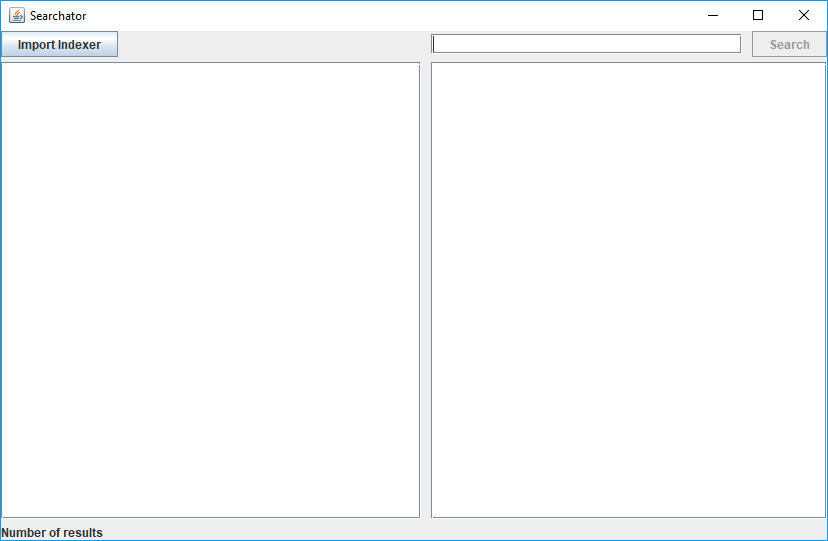
\includegraphics[width=12cm]{img/init}
	\caption{Vista de la GUI recién iniciado el programa}
	\label{fig:init}
\end{figure}

Una vez iniciado el programa solo nos permitirá importar los índices, para ello hay que pulsar en el botón y seleccionar el directorio que los contiene (Figura \ref{fig:index-folder-selection}).

\begin{figure}[H]
	\centering
	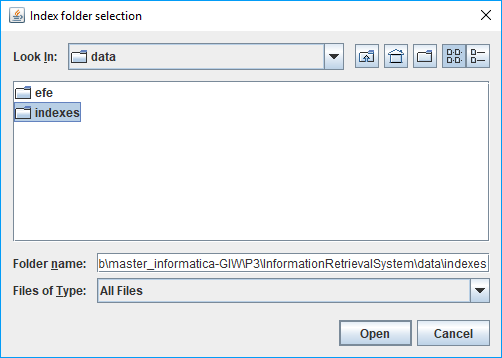
\includegraphics[width=8cm]{img/index-folder-selection}
	\caption{Selección del directorio con los índices}
	\label{fig:index-folder-selection}
\end{figure}

Ya con los índices cargados se podrán realizar búsquedas. En la izquierda aparecerán los títulos de todos los resultados encontrados, a la derecha el texto completo cuando se selecciona cualquiera de ellos y abajo a la izquierda el número de resultados y el tiempo que ha tardado en encontrarlos (Figura \ref{fig:search}).

\begin{figure}[H]
	\centering
	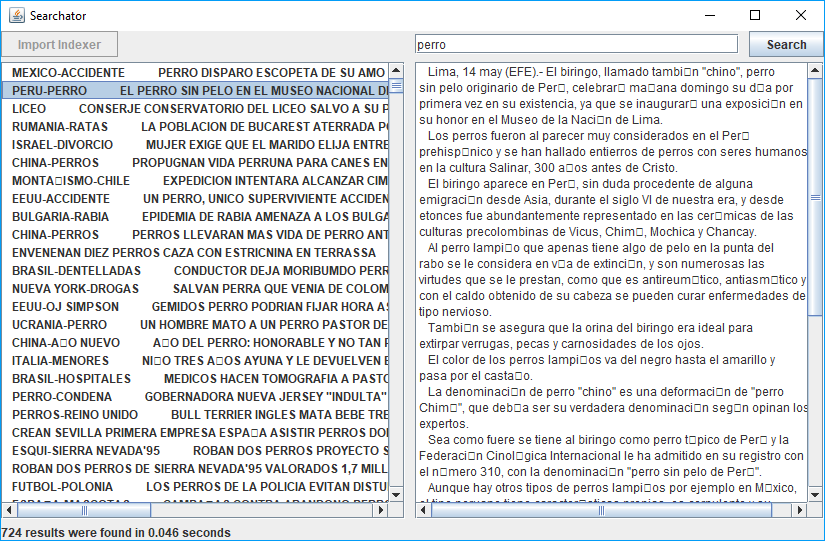
\includegraphics[width=12cm]{img/search}
	\caption{Búsqueda del término perro}
	\label{fig:search}
\end{figure}

%----------------------------------------------------------------------------------------
%	REFERENCIAS
%----------------------------------------------------------------------------------------

%\newpage

%\bibliography{referencias} %archivo referencias.bib que contiene las entradas 
%\bibliographystyle{plain} % hay varias formas de citar

\end{document}